\documentclass[aspectratio=169]{beamer}

%\includeonlyframes{current}

\usepackage[utf8]{inputenc}
\usepackage[american]{babel}
\usepackage{amsmath,amsthm}
\usepackage{unicode}
\usepackage{booktabs}
\usepackage{ifthen}
\usepackage{tikz}
\usetikzlibrary{calc,arrows,arrows.meta,intersections,positioning,decorations.pathmorphing}
\usepackage{ulem}

\mode<presentation>{%
  \usetheme{ibm}
}

\newcommand{\Z}{ℤ}
\newcommand{\F}{\mathbb{F}}
\renewcommand{\a}{\mathfrak{a}}
\renewcommand{\b}{\mathfrak{b}}
\newcommand{\g}{\mathfrak{g}}
\newcommand{\G}{\mathcal{G}}
\newcommand{\E}{\mathcal{E}}
\newcommand{\End}{\operatorname{End}}
\newcommand{\Hom}{\operatorname{Hom}}
\newcommand{\M}{\mathcal{M}}
\newcommand{\fp}{\mathrm{fp}}
\DeclareMathOperator{\rank}{rank}
\newcommand{\Cl}{\operatorname{Cl}}
\newcommand{\GL}{\operatorname{GL}}
\newcommand{\SL}{\operatorname{SL}}
\renewcommand{\O}{\mathcal{O}}

\title{Isogeny-based Crypto}
\subtitle{Coming of Age}
\author{Luca De Feo}
\date{May 13, 2026, Eurocrypt, Rome}
\institute{IBM Research Zürich}

\begin{document}

\frame[plain]{\titlepage}

%%

\begin{frame}[plain]
  \begin{tikzpicture}[overlay,remember picture]
    \draw
    (current page.center) node {\includegraphics[width=460px]{jack_frusciante.jpg}}
    +(0,-3)
    node[white,fill=black,opacity=0.3,text opacity=1,rounded corners=5] {\Huge\bf When does one become an adult?};
  \end{tikzpicture}
\end{frame}

%%

\begin{frame}{A brief history of ECC}
  \large
  \begin{description}
  \item<1->[1976] Diffie--Hellman key exchange
  \item<1->[1977] RSA
  \item<2->[1985] Miller and Koblitz introduce elliptic curves to cryptography
  \item<4->[1994] Shor's quantum algorithm
  \item<6->[1997] Couveignes' isogeny-based key exchange
  \item<3->[1999] NIST standardizes its first elliptic curves
  \item<5->[2017] NIST calls for post-quantum algorithms
  \end{description}
\end{frame}

%%

\begin{frame}
  \huge
  \begin{tikzpicture}[remember picture,overlay,shift={(current page.center)}]
    \fill[white] (8,6) rectangle (-2,-6);
    \node at (2,0) {\includegraphics[height=1.1\textheight]{cinema_paradiso}};
    \fill[ibmblue] (-8,-6) rectangle (-2,6);
    \node[white] at (-5,0.5) {High school};
    \node[white] at (-5,-0.5) {isogenies};
  \end{tikzpicture}
\end{frame}

%% 

\begin{frame}{\alt<2>{Groups}{Geometry}}
  \begin{columns}
    \begin{column}{0.5\textwidth}
      \begin{center}
        \begin{tikzpicture}[domain=-2.4566:4,samples=100,yscale=1/2]
          \draw[black!30!white] (0,-8) edge[-latex] (0,8) (-3,0) edge[-latex] (4,0);
          
          \draw plot (\x,{sqrt(\x*\x*\x-4*\x+5)});
          \draw plot (\x,{-sqrt(\x*\x*\x-4*\x+5)});

          \begin{uncoverenv}<2->
            \draw (-3,1) -- (4,8/3+3);
            \begin{scope}[every node/.style={draw,circle,inner sep=1pt,fill},cm={1,2/3,0,0,(0,3)}]
              \node at (-2.287980,0) {};
              \node at (-0.535051,0) {};
              \node at (3.267475,0) {};
            \end{scope}
            \begin{scope}[every node/.style={yshift=0.3cm},cm={1,2/3,0,0,(0,3)}]
              \node at (-2.287980,0) {$P$};
              \node at (-0.535051,0) {$Q$};
              \node at (3.267475,0) {$R$};
            \end{scope}

            \draw[dashed] (3.267475,3.267475*2/3+3) -- (3.267475,-3.267475*2/3-3) 
            node[draw,circle,inner sep=1pt,fill] {}
            node[xshift=-0.1cm,anchor=east] {$P\oplus Q$};
          \end{uncoverenv}
        \end{tikzpicture}
      \end{center}
    \end{column}
    \begin{column}{0.5\textwidth}
      \centering
      \alt<2>{
        \includegraphics[height=0.4\textheight]{galois.jpg}
        \vspace{0.05\textheight}
        \includegraphics[height=0.4\textheight]{abel.jpg}
      }{
        \includegraphics[height=0.9\textheight]{descartes.jpg}
      }
    \end{column}
  \end{columns}
\end{frame}

%%

\begin{frame}{Isogenies}
  \large\centering
  \begin{tikzpicture}
    \draw[white,font=\normalsize,
    every node/.style={rounded corners=10,fill=blue!40!white}]
    (0,0) node (E1) {$y^2 = x^3 + 1$}
    (12,0) node (E2) {$y^2 = x^3 - x$}
    (E1) edge[-latex,thick,draw=red] node[circle,fill=red!70!,above] {\Huge $φ$} (E2);

    \draw[every node/.style={anchor=west}]
    (-1,-2) node {Algebraic morphisms:~~~~
      \normalsize $\displaystyle \left(\frac{5x^2 + 5x + 4}{x + 1},\quad y\frac{2x^2 + 4x - 4}{x^2 + 2x + 1}\right)$}
    ++(0,-2) node {Group morphisms:~~~~ \normalsize $φ(P + Q) = φ(P) + φ(Q)$};

    \uncover<2->{
      \path[latex-{Bar[right,scale=3]},thick,
      every node/.style={anchor=west,blue}]
      (9,-3) node {Interpolation} edge +(-7,0)
      ++(0,-2) node {Groups \underline{\bf of} morphisms} edge +(-7,0);
    }
  \end{tikzpicture}
\end{frame}

%%

\begin{frame}{Degree}
  \begin{columns}
    \large
    \begin{column}{0.5\textwidth}
      \centering
      \[\deg(φ) \in ℕ^+\]
      \vspace{1em}
      \begin{itemize}
        \setlength{\itemsep}{2em}
      \item A measure of ``size'';
      \item<2-> \emph{Multiplicative;}
      \item<3-> A measure of ``complexity'':\\[1em]
        only isogenies of small degree fit into a computer!
      \end{itemize}
    \end{column}
    \begin{column}{0.5\textwidth}
      \centering
      \begin{tikzpicture}
        \fill[blue!50!white]
        (0,0) circle (1mm) node(A){}
        ++(2,0) circle (1mm) node(B){}
        ++(4,0) circle (1mm) node(C){};
        \draw[-latex,red]
        (A) edge[bend left] node[above]{$φ$} (B)
        (B) edge[bend left] node[above]{$ψ$} (C);

        \uncover<2->{
          \node at (3,-2) {\emph{$\deg(ψ∘φ) = \deg(ψ)\deg(φ)$}};
        }
      \end{tikzpicture}
    \end{column}
  \end{columns}
\end{frame}

%%

\begin{frame}{The isogeny problem*}
  \Large
  \vspace{\stretch{10}}
  \begin{center}
    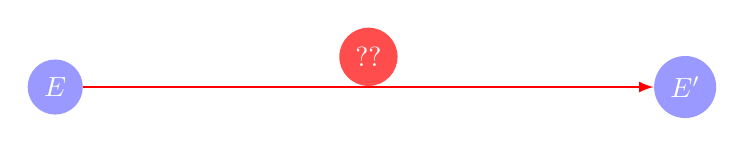
\begin{tikzpicture}
      \path[every node/.style={circle,white,fill=blue!40!white}]
      (0,0) node (E) {$E$}
      (8,0) node (E1) {$E'$};
      \uncover<2->{
        \fill[-latex,red,thick] (E) edge node[above,white,fill=red!70!white,circle] {??} (E1);
      }
    \end{tikzpicture}
  \end{center}
  
  \vspace{\stretch{15}}
  
  \normalsize *Decisional problem \underline{\bf is easy}.
\end{frame}

%%

\begin{frame}{Isogeny graphs}
  \Large
  \begin{columns}
    \begin{column}{0.45\textwidth}
      \centering
      degree
      \only<1>{$2$}%
      \only<2>{$4$}%
      \only<3>{$8$}%
      \only<4>{$16$}%
      \only<5->{$2^x$}

      \vspace{2em}
      \uncover<5->{$\to$ Isogeny \textbf{path} problem}
      \vspace{2em}
      
      \uncover<6->{
        $\to$ Hash functions\\
        (Charles, Goren, Lauter '09)
      }
    \end{column}
    \begin{column}{0.55\textwidth}
      \centering
      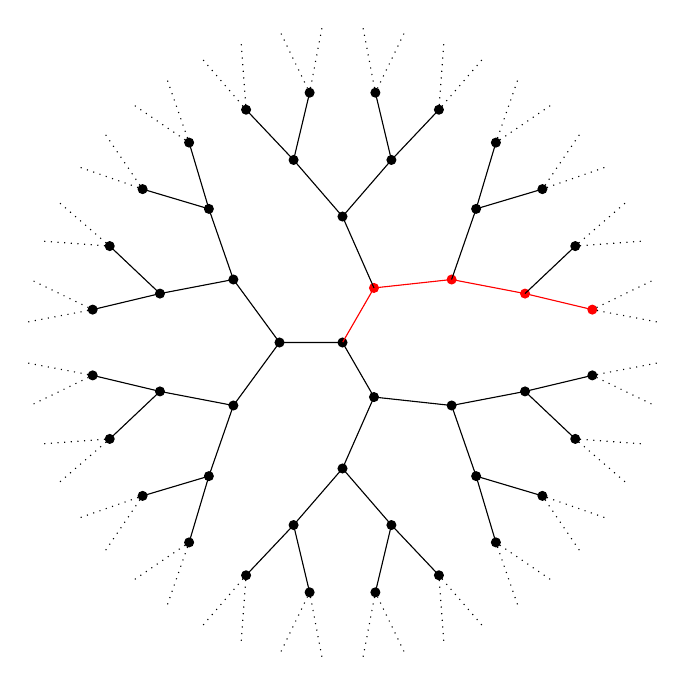
\begin{tikzpicture}[scale=0.8]
        \def\levels{5}
        \draw[fill] (0:0) circle (2pt);
        \foreach \i in {1,...,\levels} {
          \pgfmathparse{3*2^\i}
          \let\nodes\pgfmathresult
          \foreach \j in {1,3,...,\nodes} {
            \pgfmathparse{\j + (-1)^div(\j,2)}
            \let\lower\pgfmathresult
            \uncover<\i->{
              \ifthenelse{\i = \levels}{
                \draw[dotted] (360/\nodes*\j : \i) --
                (360/\nodes*\lower : \i - 1);
              }{
                \pgfextra{
                  \ifthenelse{\j=1}{\def\col{red}}{\def\col{black}}
                  \draw[fill,\col] (360/\nodes*\j : \i) circle (2pt) --
                  (360/\nodes*\lower : \i - 1);
                }
              }
            }
          }
        }
      \end{tikzpicture}
    \end{column}
  \end{columns}
\end{frame}

%%

\begin{frame}{Couveignes '97-'06 / Rostovtsev--Stolbunov '06 / CSIDH '19}
  \begin{columns}
    \begin{column}{0.55\textwidth}
      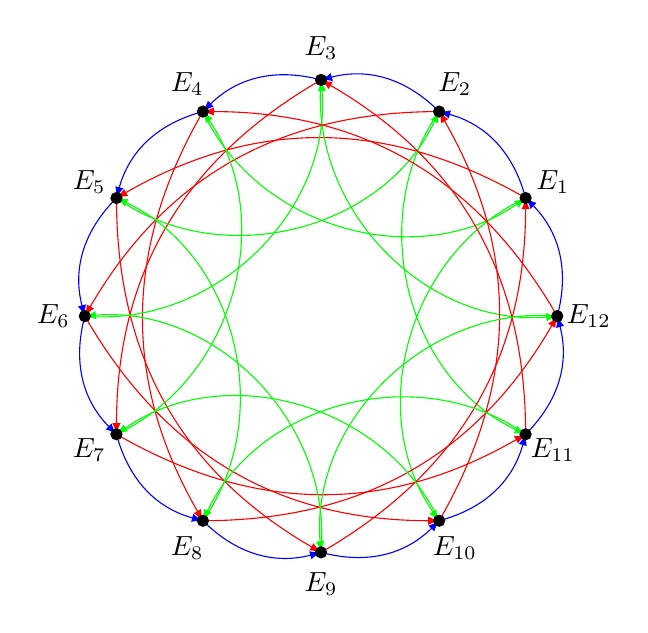
\begin{tikzpicture}
        \begin{scope}
          \def\crater{12}
          \def\jumpa{-8}
          \def\jumpb{9}
          \def\diam{3cm}

          \foreach \i in {1,...,\crater} {
            \draw[blue,-latex] (360/\crater*\i : \diam) to[bend right] (360/\crater*\i+360/\crater : \diam);
            \draw[red,-latex] (360/\crater*\i : \diam) to[bend right] (360/\crater*\i+\jumpa*360/\crater : \diam);
            \draw[green,-latex] (360/\crater*\i : \diam) to[bend right=50] (360/\crater*\i+\jumpb*360/\crater : \diam);
          }
          \foreach \i in {1,...,\crater} {
            \draw[fill] (360/\crater*\i: \diam) circle (2pt) +(360/\crater*\i: 0.4) node{$E_{\i}$};
          }
        \end{scope}
      \end{tikzpicture}
    \end{column}
    \begin{column}{0.45\textwidth}
      \large
      \begin{description}
        \setlength{\itemsep}{1em}
      \item<3->[Commutative]
        $E^{(\textcolor{red}{\bullet}\textcolor{blue}{\bullet})} = E^{(\textcolor{blue}{\bullet}\textcolor{red}{\bullet})}$
      \item<2->[Group]
        $((E^{\textcolor{blue}{\bullet}})^{\textcolor{red}{\bullet}})^{\textcolor{blue}{\bullet}} = E^{(\textcolor{blue}{\bullet}\textcolor{red}{\bullet}\textcolor{blue}{\bullet})} = E_1^{\textcolor{green}{\bullet}}$
      \item[Action]
        $E_2 = E_1^{\textcolor{blue}{\bullet}}$\\
        $E_5 = E_1^{\textcolor{red}{\bullet}}$\\
        $E_{10} = E_1^{\textcolor{green}{\bullet}}$
      \end{description}
    \end{column}
  \end{columns}
\end{frame}

%%

\begin{frame}{SIDH '11 / SIKE '17}
  \large
  \centering
  \begin{tikzpicture}
    \node (E0) at (0,0) {$E_0$};
    \node (E1) at (8,0) {$E_1$};
    \node (E2) at (0,-6) {$E_2$};
    \draw[-latex]
    (E0) edge[blue] node[above,blue] {$φ$} (E1)
    edge[red] node[left,red] {$ψ$} (E2);
    \foreach \i in {1,...,4} {
      \fill[red] ($ (E0)!\i/5!(E2) $) circle (1pt);
      \fill[blue] ($ (E0)!\i/5!(E1) $) circle (1pt);
    }
    
    \uncover<6->{
      \node (E3) at (8,-6) {$E_3$};
      \draw[-latex,blue] (E2) edge node[below] {$φ'$} (E3);
      \foreach \i in {1,...,4} {
        \fill[blue] ($ (E2)!\i/5!(E3) $) circle (1pt);
      }
    }

    \newcount\shift
    \animatevalue<2-5>{\shift}{1}{4}
    \uncover<2-5>{
      \draw[gray,-latex] ($ (E0)!\shift/5!(E2) $) to ($ (E1)!\shift/5!(E3) $);
    }
    
    \animatevalue<7-10>{\shift}{1}{4}
    \uncover<7-10>{
      \draw[gray,-latex] ($ (E0)!\shift/5!(E1) $) to ($ (E2)!\shift/5!(E3) $);
    }
    
    \uncover<11->{
      \draw[-latex,red] (E1) edge node[right] {$ψ'$} (E3);
      \foreach \i in {1,...,4} {
        \fill[red] ($ (E1)!\i/5!(E3) $) circle (1pt);
      }
    }
  \end{tikzpicture}
\end{frame}

%%

\begin{frame}[plain]
  \begin{tikzpicture}[overlay,remember picture]
    \draw
    (current page.center) node {\includegraphics[width=460px]{and_then_i_said.jpg}}
    +(0,4) node[white] {\Huge\bf AND THEN THEY SAID\dots}
    +(0,-4) node[white] {\Huge\bf OUR KEY EXCHANGE IS QUANTUM-SAFE!};
  \end{tikzpicture}
\end{frame}

%%

\begin{frame}{SQisign '20}
  \centering
  \def\pk{\mathrm{pk}}
  \def\sk{\mathrm{sk}}
  \def\comm{\mathrm{com}}
  \def\chal{\mathrm{chl}}
  \def\resp{\mathrm{rsp}}
  \def\aux{\mathrm{aux}}
  \begin{tikzpicture}[scale=1.5]
    \begin{scope}[gray]
      \node at (0, 0) (E0) {$E_{0}$};
      \node at (2, 0) (Epk) {$E_\pk$};
      \node at (-1, -2) (Ecomm) {$E_\comm$};
      \node at (3, -2) (Echl0) {$E_\chal^0$};
      \node at (3.5, -3) (Echl) {$E_\chal$};
      \node at (1.5, -2) (Echlpr) {$E_\chal'$};
      \node at (1.5, -4) (Eauxpr) {$E_\aux'$};
      \node at (-1, -4) (Eaux) {$E_\aux$};
      \draw[-latex] (E0) -- (Epk)  node[midway, above] (phi_sk) {$\varphi_{\sk}$};
      \draw[-latex] (E0) -- (Ecomm)  node[midway, left] (phi_com) {$\varphi_{\comm}$};
      \draw[-latex] (Epk) -- (Echl0)  node[midway, left] (phi_chl1) {$\varphi_{\chal}'$};
      \draw (Epk) edge[-latex, bend left] (Echl);
      \node at (3.7, -1.2) (phi_chl) {$\varphi_\chal$};
      \draw[-latex] (Echl0) -- (Echl)  node[midway, left] (back) {$\empty$};
      \draw[-latex] (Ecomm) -- (Echlpr)  node[midway, above] {$\varphi_\resp^{(1)}$};
      \draw[-latex] (Echlpr) -- (Echl0)  node[midway, above] (phi_rsp0) {$\varphi_\resp^{(0)}$};
      \draw[-latex] (Ecomm) -- (Eaux)  node[midway, left] {$\varphi_\aux$};
      \draw[-latex] (Echlpr) -- (Eauxpr)  node[midway, right] {$\varphi_\aux'$};
      \draw (Eaux) edge[-latex, dotted] (Eauxpr);
      \draw (0.25,-3) node[scale=1.8] (commute) {$\circlearrowright$};
    \end{scope}
    
    \begin{scope}[->,thick]
      \large
      \uncover<+->{
        \node at (5,0) {isogeny walk} edge[bend left] (phi_chl)
        edge[bend right] (phi_chl1)
        edge (phi_rsp0);
      }
      \uncover<+->{
        \node at (-3,-1) {quaternionic ideal} edge[bend right] (phi_com)
        edge[bend left] (phi_sk);
      }
      \uncover<+->{
        \node at (4,-4) {backtracking walk} edge[bend left] (back);
      }
      \uncover<+->{
        \node at (-3,-2) {HD representation} edge[bend right] (commute);
      }
      \begin{scope}[every node/.style={rounded corners=10,decorate,inner sep=1em},
        decoration={snake}]
        \uncover<+->{
          \node[rotate=30,blue,fill=yellow] at (0,-1) {\Large Deuring correspondence};
        }
        \uncover<+->{
          \node[rotate=-20,red,fill=green] at (-2,-1) {\Large Theta structures};
        }
        \uncover<+->{
          \node[rotate=0,white,fill=magenta] at (3,0) {\Large Kani's lemma};
        }
        \uncover<+->{
          \node[rotate=50,green,fill=pink] at (3,-2) {\huge Clapoti};
        }
        \uncover<+->{
          \node[rotate=-80,yellow,fill=purple] at (0,-3) {\huge KlaPoTi};
        }
        \uncover<+->{
          \node[rotate=0,teal,fill=orange] at (1, -2) {\Huge Qlapoti};
        }
      \end{scope}
    \end{scope}
  \end{tikzpicture}
  
  \footnotetext[1]{From \textit{``SQIsign2D–West: The Fast, the Small, and the
      Safer''}, Asiacrypt 2024.}
\end{frame}

%%

\begin{frame}[plain]
  \begin{tikzpicture}[overlay,remember picture]
    \draw
    (current page.center) +(0,-1) node {\includegraphics[width=460px]{pepe_silvia.jpg}}
    +(0,-4) node[white] {\Huge\bf IT'S FUNCTORIAL, BRUH!!1!};
  \end{tikzpicture}
\end{frame}

%%

\begin{frame}{Too small to fail}
  \centering
  \textbf{SQIsign v2 (June 2025)}
  \begin{table}[h]
    \centering
    \begin{tabular}{c r r r r r}
      \toprule
      & \multicolumn{2}{c}{Sizes (bytes)} & \multicolumn{3}{c}{Timings (ms)}\\
      \cmidrule(lr){2-3}\cmidrule(lr){4-6}
      Security & Public Key & Signature & Keygen & Sign & Verify \\
      \midrule
        NIST-1 &  66 & 148 &  25 &   60 &  3 \\
        NIST-3 &  98 & 222 &  67 &  161 &  9 \\
        NIST-5 & 130 & 294 & 119 &  300 & 18 \\
      \bottomrule
    \end{tabular}
  \end{table}
\end{frame}

%%

\begin{frame}
  \huge
  \begin{tikzpicture}[remember picture,overlay,shift={(current page.center)}]
    \fill[white] (8,6) rectangle (-2,-6);
    \node at (3,0) {\includegraphics[height=1.1\textheight]{per_qualche_dollaro}};
    \fill[ibmblue] (-8,-6) rectangle (-2,6);
    \node[white] at (-5,0.5) {Technical};
    \node[white] at (-5,-0.5) {slides ahead};
  \end{tikzpicture}
\end{frame}

%%

\begin{frame}{Algebraic geometry: the classical PoV (\dots--1930's)}
  \large
  \begin{columns}
    \begin{column}{0.65\textwidth}
      \centering
      \[
        \begin{array}{c c c c c c c }
          x^2 & + 3y^2 & + xy & + 10x & -7y & +4 & = 0\\
          x^2 & - y^2 & + xy & + 9x & -y & -3 & = 0\\
                 & - 2y^2 &  & -3x & -8y & +9 & = 0\\
          x^2 & + y^2 & + 13xy & + 10x & -7y &  & = 0\\
          x^2 & - 5y^2 & + xy & + 10x & +11y & +3 & = 0\\
          x^2 & + y^2 & + 11xy & - 8x & +6y &  & = 0\\
          x^2 &  &  &  & -9y & +4 & = 0\\
        \end{array}
      \]
    \end{column}
    \begin{column}{0.35\textwidth}
      \centering
      \begin{itemize}
        \setlength{\itemsep}{1em}
      \item Syzygies
        \begin{itemize}
        \item Gröbner bases
        \item Distinguishers for codes
        \end{itemize}
      \item Invariants
        \begin{itemize}
        \item Tensors
        \item Exterior algebra
        \item Moduli spaces
        \end{itemize}
      \item \dots
      \end{itemize}
    \end{column}
  \end{columns}
\end{frame}

%%

\begin{frame}{Algebraic geometry: the modern PoV (1930's--\dots)}
  \large
  \begin{columns}
    \begin{column}{0.5\textwidth}
      \centering
      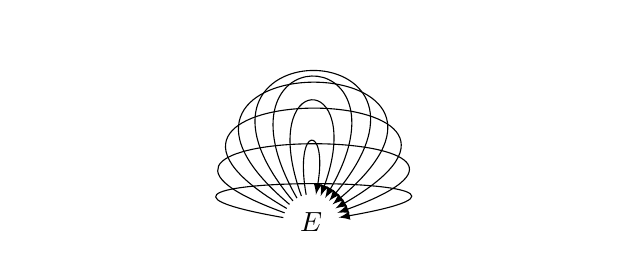
\begin{tikzpicture}
        \fill (0,-1) node[circle](A){$E$};
        \foreach  \i in {1,...,8} {
          \draw[-latex] (A) edge[loop,out=90+10*\i,in=90-10*\i,looseness=20-\i] (A);
        }
      \end{tikzpicture}
    \end{column}
    \begin{column}{0.5\textwidth}
      \[\emph{(φ+ψ)}(P) := φ(P) + ψ(P)\]
      \bigskip
      \[\emph{(φ∘ψ)}(P) := φ(ψ(P))\]
      \bigskip
      \[\emph{φ∘(ψ+χ) = φ∘ψ + φ∘χ}\]
    \end{column}
  \end{columns}
\end{frame}

%%

\begin{frame}{Endomorphism rings}
  \large\centering
  \begin{tikzpicture}
    \node at (-1,0) {$ℚ(\sqrt{-p})$};
    \uncover<2->{
      \node at (1,0) {$ℚ(\sqrt{-q})$};
    }
    \uncover<3->{
      \draw (0,-2) ellipse (7cm and 2.5cm);
      \node at (1,-3) {$ℚ(\sqrt{-r})$};
      \node at (-5,-3) {\normalsize $ℚ(\sqrt{-s})$};
      \node at (-1.5,-2.5) {\small $ℚ(\sqrt{-t})$};
      \node at (5,-2) {\small $ℚ(\sqrt{-t})$};
      \node at (0,-1) {\footnotesize $ℚ(\sqrt{-u})$};
      \node at (3,-1.5) {\tiny $ℚ(\sqrt{-v})$};
      \node at (-3,-1) {\normalsize $ℚ(\sqrt{-w})$};
      \node at (4,-3.5) {\small $ℚ(\sqrt{-z})$};
    }

    \uncover<1>{\node at (0,-5) {Quadratic imaginary field};}
    \uncover<2->{\node at (0,-6) {\emph{$i^2 = -p\qquad j^2 = -q\qquad ij = -ji$}};}
    \uncover<3->{\node at (0,-5) {Quaternion algebra};}
  \end{tikzpicture}
\end{frame}

%%

\begin{frame}
  \large\centering
  \begin{tikzpicture}
    \useasboundingbox (-2,3) rectangle (12,-4);
    \path[circle]
    (0,-1) node(A){$E_0$}
    (4,-1) node(B){\only<2->{$E$}};

    \foreach  \i in {1,...,8} {
      \draw[-latex] (A) edge[loop,out=90+10*\i,in=90-10*\i,looseness=20-\i] (A);
      \uncover<2->{\draw[-latex,red] (B) edge[bend left=10*\i] (A);}
      \pgfmathtruncatemacro\s{\i+2}
      \uncover<\s->{\draw[-latex] (B) edge[loop,out=90+5*\i,in=90-5*\i,looseness=20-\i] (B);}
    }

    \begin{scope}[shift={(9,0)},scale=0.5]
      \node at (0,-7) {$ℤ[\sqrt{-q}]$};
      \clip (-5.5,-5.5) rectangle (5.5,5.5);
      \draw[black!20!white] (-5,0) -- (5,0) (0,-5) -- (0,5);
      \foreach \i in {-5,-2.5,...,5} {
        \foreach \j in {-5,...,5} {
          \fill[gray] (\j,\i) circle (2pt);
        }
      }
      \uncover<1>{
        \path[latex-] (0,2.5) node[above] {\small $\sqrt{-q}$} edge (0,0)
        (1,0) node[right] {\small $1$} edge (0,0);
      }
      \uncover<2->{
        \path[-latex,red,thick] (0,0) edge (2,5) edge (3,0);
        \foreach \i in {-1,...,1} {
          \foreach \j in {-2,...,2} {
            \fill[red] (\i*2+\j*3,\i*5) circle (4pt);
          }
        }
      }
    \end{scope}
    
    \uncover<12->{
      \begin{scope}[decoration={random steps,segment length=1mm,amplitude=0.1mm},thick]
        \draw[decorate] (4.4,-0.9) -- ++(0.5,-0.2) -- ++(-0.55,-0.2);
        \draw[decorate] (1.8,-2.5) -- ++(0,-1.2) edge +(0.1,0) edge +(0.1,0.05);
        \draw[decorate] (2,-2.5) -- ++(0,-1.2) edge +(0.1,0) edge +(0.1,0.05);
      \end{scope}
    }
  \end{tikzpicture}

  \uncover<11->{
    \begin{center}
      \emph{Deuring:} $\End(E_0)$-lattices are in 1-to-1 correspondence with curves isogenous to $E_0$.
    \end{center}
  }
\end{frame}

%%

\begin{frame}{Class group action (Complex multiplication)}
  \centering\large
  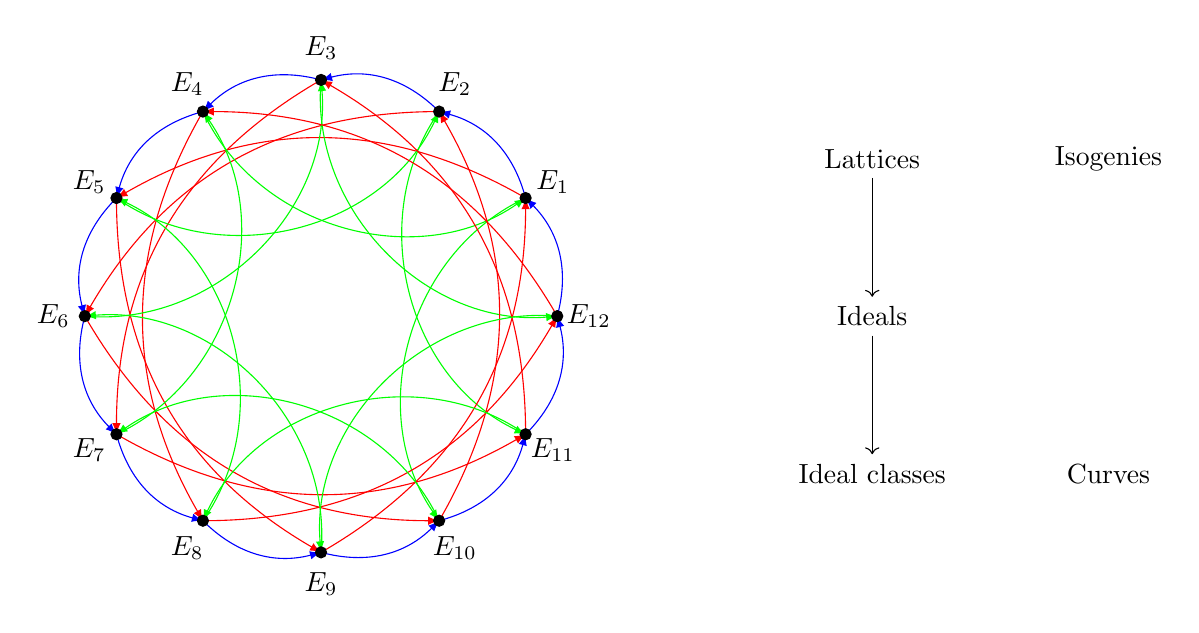
\begin{tikzpicture}
    \begin{scope}
      \def\crater{12}
      \def\jumpa{-8}
      \def\jumpb{9}
      \def\diam{3cm}

      \foreach \i in {1,...,\crater} {
        \draw[blue,-latex] (360/\crater*\i : \diam) to[bend right] (360/\crater*\i+360/\crater : \diam);
        \draw[red,-latex] (360/\crater*\i : \diam) to[bend right] (360/\crater*\i+\jumpa*360/\crater : \diam);
        \draw[green,-latex] (360/\crater*\i : \diam) to[bend right=50] (360/\crater*\i+\jumpb*360/\crater : \diam);
      }
      \foreach \i in {1,...,\crater} {
        \draw[fill] (360/\crater*\i: \diam) circle (2pt) +(360/\crater*\i: 0.4) node{$E_{\i}$};
      }
    \end{scope}

    \begin{scope}[shift={(7,2)}]
      \path
      (0,0) node (A) {Lattices} +(3,0) node (D) {Isogenies}
      ++(0,-2) node (B) {Ideals} 
      ++(0,-2) node (C) {Ideal classes} +(3,0) node (E) {Curves}
      (A) edge[->] (B)
      (B) edge[->] (C)
      ($(A)!0.5!(D)$) node {$\circlearrowright$}
      ($(C)!0.5!(E)$) node {$\circlearrowright$};
    \end{scope}
  \end{tikzpicture}
\end{frame}

%%

\begin{frame}{Grupoid action (Quaternionic multiplication)}
  \centering\large
  \begin{center}
    \emph{Grupoid} = group with ``partial'' multiplication
  \end{center}

  \bigskip
  
  \begin{tikzpicture}
    \fill[circle]
    (0,0) node (A) {} circle (2pt)
    (3,2) node (B) {} circle (2pt)
    (6,0) node (C) {} circle (2pt);
    \path[-latex]
    (A) edge node[auto] {$a$} (B) edge node[auto,swap] {$c = ab$} (C)
    (B) edge node[auto] {$b$} (C)
    (A) edge[loop left] (A)
    (B) edge[loop above] (B)
    (C) edge[loop right] (C);
  \end{tikzpicture}
\end{frame}

%%

\begin{frame}
  \Huge\centering
  \begin{tikzpicture}
    \useasboundingbox (-5,-2) -- (5,2);
    \path
    (0,0) node {$\circlearrowright$}
    (-4,0) node {\alt<2->{Algebra}{(Ideal) Lattices}}
    (4,0) node {\alt<2->{Geometry}{Curves}};
  \end{tikzpicture}
\end{frame}

%%

\begin{frame}{Identification Schemes from Group(oid) Actions}
  \large
  \begin{columns}
    \begin{column}{0.5\textwidth}
      \centering
      \begin{tikzpicture}
        \node (E0) at (0,0) {$E_0$};
        \node (Epk) at (6,0) {$E_{\mathrm{pk}}$};
        \uncover<2->{
          \node (Ecom) at (3,-5) {$E_{\mathrm{com}}$};
        }

        \draw[dashed,-latex]
        (E0) edge node[above]{{\small secret key:}~~~~\emph{$σ$}} (Epk);
        
        \uncover<2-3>{
          \draw[dashed,-latex]
          (E0) edge node[below,sloped]{\emph{$π$}~~~~\small random} (Ecom);
        }

        \uncover<3>{
          \draw[-latex] (E0) edge (Ecom);
        }

        \uncover<4->{
          \draw[-latex] (Epk) edge node[below,sloped]{\emph{$σ^{-1}π$}} (Ecom);
        }
      \end{tikzpicture}
    \end{column}
    \begin{column}{0.5\textwidth}
      \begin{description}
        \setlength{\itemsep}{1em}
      \item[Graph isomorphism:] Goldreich, Micali, Widgerson 1992;
      \item[Class group action:] Couveignes 1997 / Stolbunov 2008;
      \item[Quaternionic multiplication:] Galbraith, Petit, Silva 2016;
      \item[Code equivalence:] Biasse, Micheli, Persichetti, Santini
        2020;
      \end{description}
    \end{column}
  \end{columns}
\end{frame}

%%

\begin{frame}
  \huge
  \begin{tikzpicture}[remember picture,overlay,shift={(current page.center)}]
    \fill[white] (8,6) rectangle (-8,-2);
    \node at (0,0.7) {\includegraphics[width=1.1\textwidth]{ben_hur}};
    \fill[ibmblue] (-8,-6) rectangle (8,-2);
    \node[white] at (0,-3) {Coming soon};
  \end{tikzpicture}
\end{frame}

%%

\begin{frame}{How general (or not) is SQIsign?}
  \Large\centering
  
  Beyond groupoids: axiomatizing SQIsign

  \bigskip
  
  \large joint work with Basso, Patranabis, Radulescu, Wesolowski
\end{frame}

%%

\begin{frame}{Higher dimensional abelian varieties}
  \centering
  \begin{tikzpicture}[domain=-2.4566:4,samples=100]
    \begin{scope}[xscale=0.3,yscale=0.5]
      \draw plot (\x,{sqrt(\x*\x*\x-4*\x+5)});
      \draw plot (\x,{-sqrt(\x*\x*\x-4*\x+5)});
      \node (P1) at (3,4.47213595499958) {};
    \end{scope}
    \begin{scope}[xscale=0.7,yscale=0.15,shift={(7,-20)}]
      \draw plot ({sqrt(\x*\x*\x-4*\x+5)},\x);
      \draw plot ({-sqrt(\x*\x*\x-4*\x+5)},\x);
      \node (P2) at (-4.47213595499958,3) {};
    \end{scope}
    \node at (5,0) {\huge $E×E$};
    
    \fill (P1) circle (2pt);
    \fill (P2) circle (2pt);

    \draw[dashed] (P2) -- (P2 |-, |- P1) -- (P1);
    \fill (P2 |-, |- P1) circle (2pt) node[above right] {$(P,Q)$};
  \end{tikzpicture}
\end{frame}

%%

\begin{frame}{HD-mania}
  \centering\large
  \begin{tikzpicture}
    \path
    (0,0) node {\includegraphics[width=0.7\textwidth]{wouter-ec}}
    ++(7.5,1) node {\includegraphics[width=0.3\textwidth]{wouter-ec-qr}}
    ++(0,-2.5) node {\emph{\url{youtu.be/CpqjkfuXeoQ}}};
  \end{tikzpicture}
\end{frame}

%%

\begin{frame}{$\otimes$-MIKE (Robert \textit{et ignoti}) ~~~ {\small(\url{ia.cr/2024/1556})} }
  \Huge\centering
  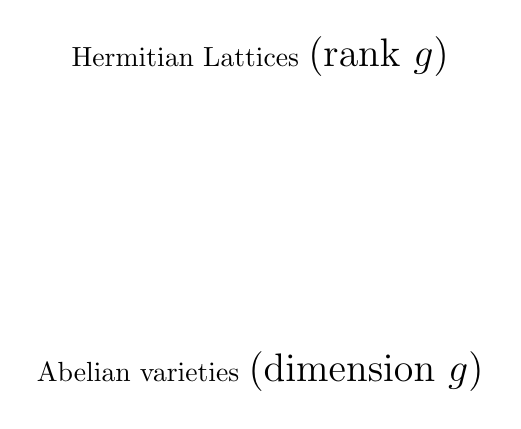
\begin{tikzpicture}
    \path
    (0,0) node {$\circlearrowright$}
    (0,2) node {Hermitian Lattices \Large(rank $g$)}
    (0,-2) node {Abelian varieties \Large(dimension $g$)};
  \end{tikzpicture}
\end{frame}

%%

\begin{frame}
  \huge
  \begin{tikzpicture}[remember picture,overlay,shift={(current page.center)}]
    \fill[white] (-8,6) rectangle (8,-1);
    \node at (0,2) {\includegraphics[width=1.1\textwidth]{la_grande_bellezza}};
    \fill[ibmblue] (-8,-6) rectangle (8,-1);
    \node[white] at (0,-2.5) {FAQ};
  \end{tikzpicture}
\end{frame}

%%

\begin{frame}{Aren't isogenies broken anyway?}
  \Large
  As much as:
  \bigskip
  \begin{description}
    \setlength{\itemsep}{1em}
  \item[ECC:] MOV pairing attack
  \item[Lattices:] Basically any signature before Fiat--Shamir w aborts
  \item[Codes:] Signatures, Syzygy distinguishers
  \item[Multivariate:] HFE, Rainbow
  \end{description}
\end{frame}

%%

\begin{frame}{Do I need to study the EGA to understand isogenies?}
  \Large\centering
  \begin{tikzpicture}
    \useasboundingbox (0,3) -- (6,-3);
    \path
    (0,0) node {\includegraphics[height=0.8\textheight]{ega}}
    (4,0) node[anchor=west] {No. \only<2->{But it won't hurt you.}};
  \end{tikzpicture}
\end{frame}

%%

\begin{frame}{When are you going to write a book?}
  \huge\centering
  \uncover<2->{Next question!}
\end{frame}

%%

\begin{frame}
  \huge
  \begin{tikzpicture}[remember picture,overlay,shift={(current page.center)}]
    \fill[white] (8,6) rectangle (-2,-6);
    \node at (4,0) {\includegraphics[height=1.1\textheight]{vacanze_romane}};
    \fill[ibmblue] (-8,6) rectangle (-2,-6);
    \node[white] at (-5,0) {Community};
  \end{tikzpicture}
\end{frame}

%%

\begin{frame}
  \centering
  \begin{tikzpicture}
    \path
    (0,0) node {\includegraphics[width=8cm]{isogeny-club}}
    (0,4) node {\includegraphics[width=8cm]{isogeny-club-logo}}
    (8,2) node {\includegraphics[width=4cm]{isogeny-club-qr}}
    ++(0,-3) node {\url{https://isogeny.club}};
  \end{tikzpicture}
\end{frame}

%%

\begin{frame}
  \huge
  \begin{tikzpicture}[remember picture,overlay,shift={(current page.center)}]
    \fill[white] (8,6) rectangle (-8,-1);
    \node at (0,1) {\includegraphics[height=1.1\textheight]{i_soliti_ignoti}};
    \fill[ibmblue] (-8,-1) rectangle (8,-6);
    \node[white] at (0,-2.5) {Famous last words};
  \end{tikzpicture}
\end{frame}

%%

\begin{frame}
  \Huge\centering
  \begin{tikzpicture}
    \useasboundingbox (-5,-2) -- (5,2);
    \path
    (0,0) node {$\circlearrowright$}
    (-3,0) node {Algebra}
    (3,0) node {Geometry};
  \end{tikzpicture}
\end{frame}

%%

\begin{frame}[plain,]
  \large
  \begin{tikzpicture}[remember picture,overlay,shift={(current page.center)}]
    \node at (0,0) {\includegraphics[width=1.1\textwidth]{domino}};
    \begin{scope}[white]
      \node at (-1,-4.2) {Diffie--Hellman};
      \node at (-2,-3.7) {Class Group Actions};
    \end{scope}
    \node at (-0.3,-1.8) {SIDH};
    \node at (-1.1,-0.5) {SQIsign};
    \node at (-2,1.3) {SQIsignHD};
    \node at (-3.5,3) {$\otimes$-MIKE};
  \end{tikzpicture}
\end{frame}

%%

\begin{frame}[plain,]
  \centering
  \begin{tikzpicture}
    \path
    (0,3.5) node {\includegraphics[width=7cm]{sqisign-logo}}
    (0,0.5) node{\Huge\bf Thank you}
    (0,-0.6) node{\large\url{https://defeo.lu/}}
    (0,-1.3) node{\large\includegraphics[height=0.9em]{mastodon.png}~\href{https://twitter.com/luca_defeo}{@luca\_defeo@ioc.exchange}}
    (0,-1.9) node{\large\includegraphics[height=0.9em]{bluesky.png}~\href{https://bsky.app/profile/bsky.defeo.lu}{@bsky.defeo.lu}};
  \end{tikzpicture}
\end{frame}

\end{document}


% LocalWords:  Isogeny abelian isogenies hyperelliptic supersingular Frobenius
% LocalWords:  isogenous
